\documentclass[11pt,compsoc]{IEEEtran}
\usepackage[spanish]{babel}
\usepackage{amsmath,amsfonts}
\usepackage{algorithmic}
\usepackage{array}
\usepackage[caption=false,font=normalsize,labelfont=sf,textfont=sf]{subfig}
\usepackage{textcomp}
\usepackage{stfloats}
\usepackage{url}
\usepackage{verbatim}
\usepackage{graphicx}
\hyphenation{op-tical net-works semi-conduc-tor IEEE-Xplore}
\def\BibTeX{{\rm B\kern-.05em{\sc i\kern-.025em b}\kern-.08em
		T\kern-.1667em\lower.7ex\hbox{E}\kern-.125emX}}
\usepackage{balance}
\begin{document}
	\title{El procesador CELL, desde un enfoque
		histórico}
	\author{Ramiro Barcala Roca, Valentin Angrigiani, Gabriel Hackl}
		
	\markboth{Organizacion del Computador, Catedra Marchi, 2024}%
	{How to Use the IEEEtran \LaTeX \ Templates}
	\maketitle
	
	\begin{abstract}
		Este trabajo tratará el procesador CELL de Sony. Se toma un enfoque investigativo y contrastante entre arquitecturas del CELL, y otras de la época (y la actualidad). Las aplicaciones principales para las que fue diseñado, y las aplicaciones que se descubrieron luego junto  con su importancia histórica. Conceptos básicos de computación heterogénea (distintos nucleos). Analisis a futuro relacionandolo a todo.
	\end{abstract}
	
	\begin{IEEEkeywords}
		SPE,PPE,SIMD,Pipeline-ing, paralelismo, calculos vectoriales, computacion heterogenea.
	\end{IEEEkeywords}
	
	\section{Introducción}
	\IEEEPARstart{A} mediados de los 2000, la empresa Sony empieza a investigar y desarrollar su sistema de entretenimiento "Play-Station 3". Todo esto en un mercado competitivo frente a otras marcas como Microsoft y Nintendo. Terminan con un procesador multi-core, el cual tiene como particularidades los sub-nucleos. Sony tambien quería estandarizar su procesador en dispositivos de todas las gamas y usos multimedias.
	
	Sin embargo, tanto el producto como su procesador,fueron un fracaso comercial. Sin embargo, se descubrieron usos investigativos/científicos/economicos, entre otros.
	
	
	\section{Epoca Pre-CELL}
	\noindent Para ponernos en contexto, vamos a explicar la situacion de las arquitecturas del momento, como de las empresas que lanzaban nuevos productos (del mismo rubro o parecido), en aquella época.
	
	\subsection{Empresas del rubro de las consolas}
	\noindent 
	En el año 2005, las siguientes empresas de consolas/videojuegos, competian en el mercado: 
	\begin{itemize}
		\item{{\bf{Sony}}: parte de un exito rotundo con su anterior producto: la PS2. Tenia grandes expectativas con su nuevo producto, apuesta a lo grande, con nuevas funcionalidades no esenciales (ej: puertos HDMI, Blue-Ray, etc).}
		
		\item{{\bf{Microsoft}}: viene de un exito modesto, con su primer producto: la X-Box. En la X-Box 360, se centra en abaratar su producto, pero proveer servicios en linea de gran calidad. Esto les pasa factura con los problemas de hardware que tendria la consola mas adelante.}
		
		\item{{\bf{Nintendo}}: tuvo un exito pobre en su consola anterior, la Gamecube. En la Wii, se decide no hacer costos de fabricacion muy caros. Pero además, se centra en facilitar experiencias novedosas para el usuario final, mediante el uso de movimientos corporales para controlar los juegos, como extensiones al mismo control (volantes, soportes, etc).}
	\end{itemize}
	Para comprender un poco mas la magnitud del la importancia del mercado, los siguiente graficos muestran como alrededor de esos años, la industria de los videojuegos crece de una manera formidable, tanto como la porcion del mercado de cada empresa.
	
	\begin{center}
		{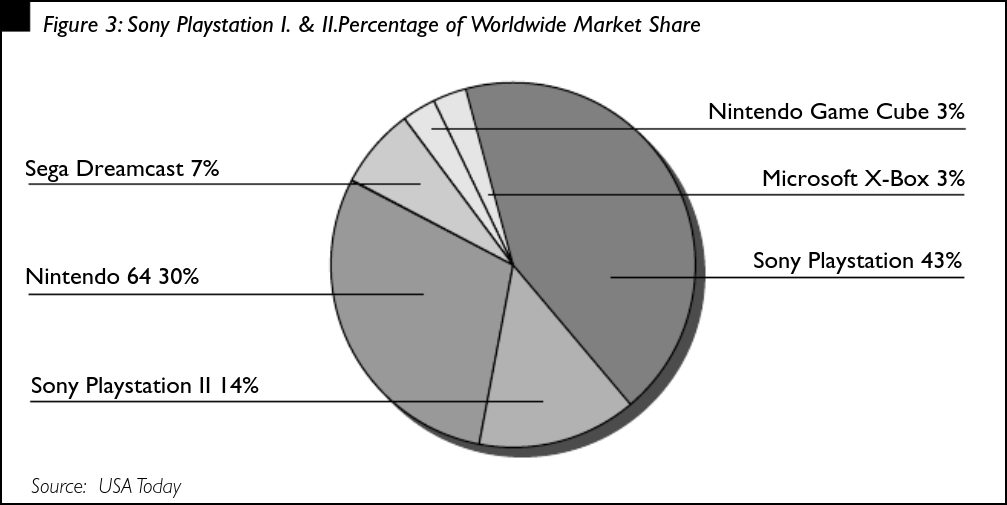
\includegraphics[width=3in,height=2in,clip,keepaspectratio]{imgs/marketshare.png}}\newline\newline
		{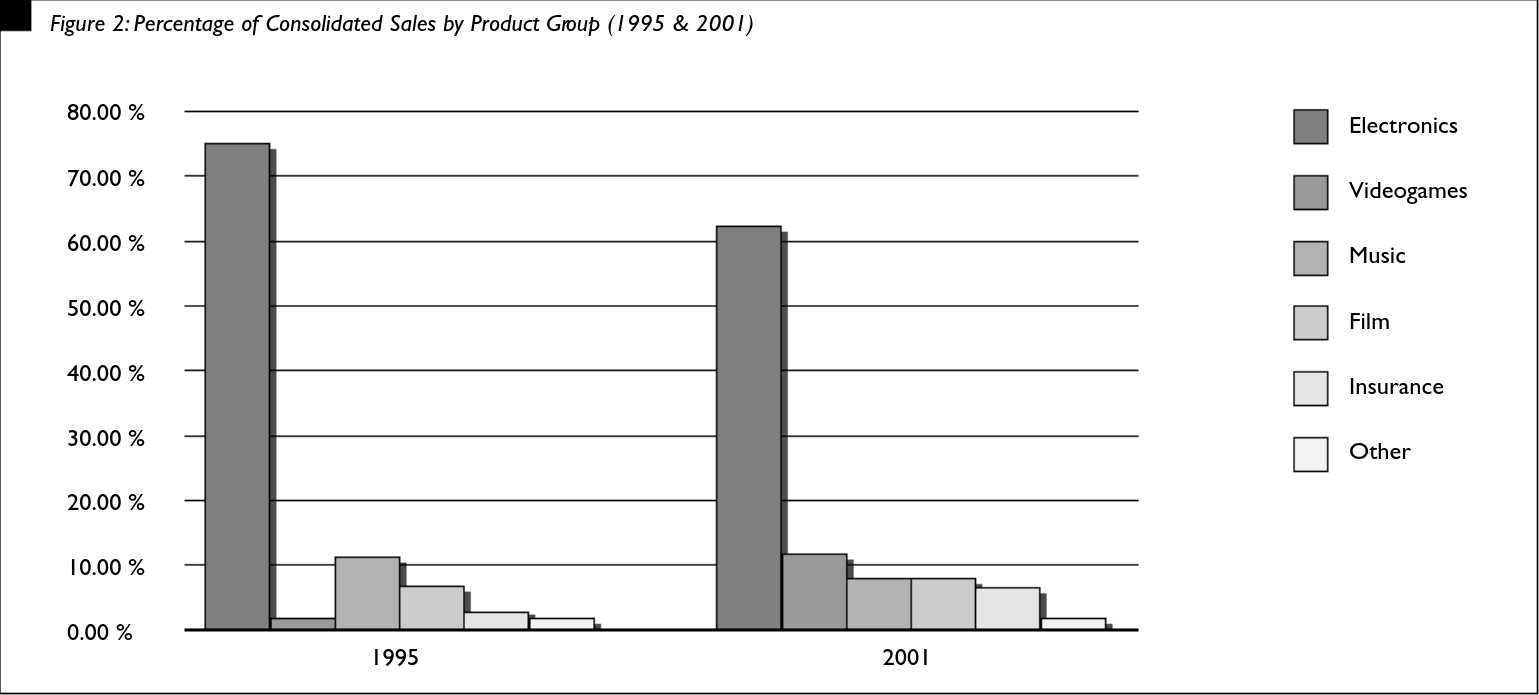
\includegraphics[width=3in,height=2in,clip,keepaspectratio]{imgs/gamingshare.png}}
	\end{center}
	
	
	\section{Arquitectura CELL}	% MODULOS,ARQUITECTURAS INTERNAS, CONVENCIONES, INSTRUCCIONES, etc
	\noindent Diseñada por Sony, en conjunto con Toshiba e IBM, esta arquitectura trae al mercado un procesador que maneja fuertemente la computacion heterogenea, mediante el uso de sus 9 nucleos. 
	
	Si bien originalmente se pensaba incluirlo en dispositivos multimedia y del entretenimiento varios, se termino destinando casi unicamente en la PS3.\newline
	
	\begin{center}
		{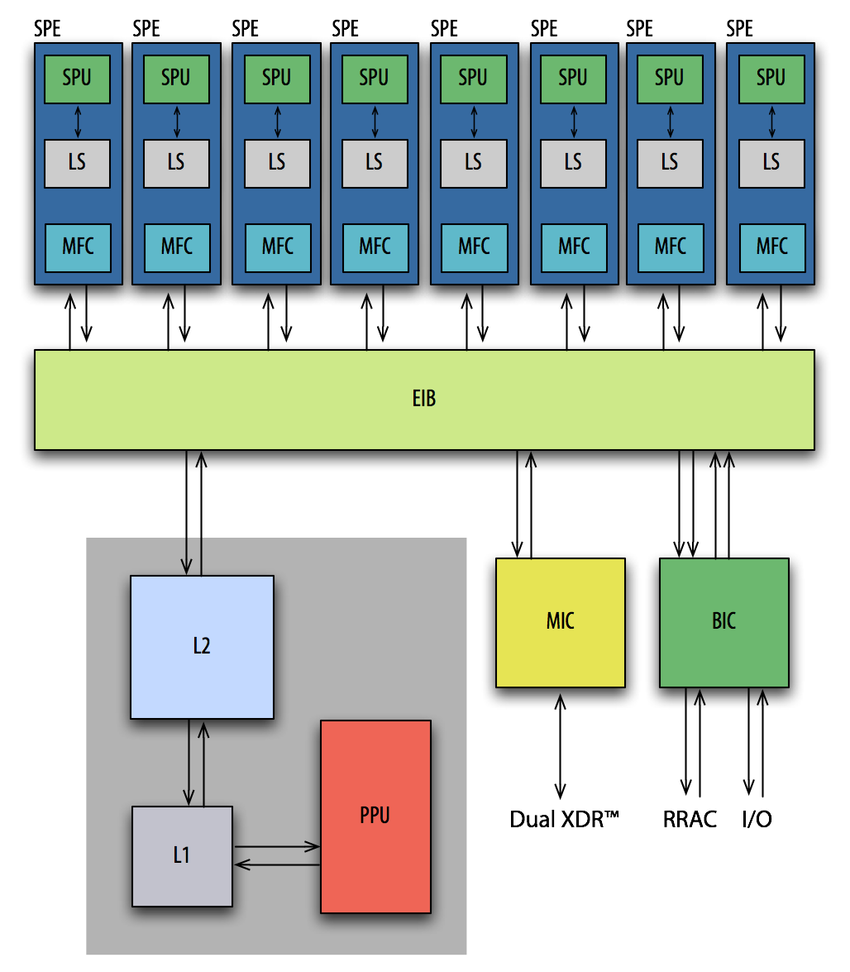
\includegraphics[width=4in,height=4in,clip,keepaspectratio]{imgs/arquitecturacell.png}}\newline
	\end{center}
	
	
	\subsection{Distintos modulos del Cell} 
	\noindent Para empezar, hablaremos del PPE (Power Processing Element). Este nucleo, es el principal de la arquitectura. Es de proposito general, y a su vez se encarga de controlar el resto de los sub-nucleos (cargar memoria y ejecutar instrucciones).
	
	Estaba conformado por 2 niveles de memoria caché, y un PPU (Power Processing Unit).\newline
	
	Luego, los SPE (Synergistic Processor Element), son los distintos sub-nucleos de la arquitectura. No son de proposito general, mas bien se encargan de realizar operaciones vectoriales, dirigidas desde el PPE. Cada uno tiene su memoria interna (Local Store), y un modulo Memory Flow Controller para poder recibir/transmitir datos desde el Bús, y un SPU (Synergistic Processing Unit).
	Trabajan con instrucciones SIMD con punto flotante, pudiendo llegar a realizar 25,6Gflops por segundo (25,6 mil millones de operaciones de punto flotante/s), por cada SPE. Vale la pena mencionar que las instrucciones SIMD se encargan de aplicar la misma operacion a un conjunto de datos, para asi poder obtener un mayor rendimiento en tiempo.\newline
	
	\subsection{Interconexion} 
	\noindent La interconexion de los distintos modulos y nucleos (ademas de la memoria externa, y la interfaz I/O) se realizaba mediante el Element Interconnection Bus. Dicho bus estaba conformado por 4 anillos unidireccionales tokenizados, 2 en cada direcciones. Era un bus tokenizado, por ende la informacion no se retransmitia mas de lo que debia, mediante un identificador del modulo al que debia llegar la informacion. 
	Por como estaba armado, nunca seria posible saturar dicho bus (ancho de banda interno maximo de 204,8GB/s).
	
	\subsection{Computacion heterogenea en el Cell }% SIMD
	\noindent La computacion heterogenea puede ser entendida como aquella computacion que requiere el manejo y codificado de instrucciones para una arquitectura que use distintos tipos de nucleos.\newline
	
	 Resulta que la computacion heterogenea, en el Cell, se aplica a los distintos SPE que residen en el mismo. De forma, que no solo programamos el PPE, sino los SPE, los cuales reciben sus instrucciones (y memoria cargada) del anterior mencionado. Ademas, el propio desarrollador puede realizar cierto tipo de pipelining; Paralelizar los programas de los SPE,vectorizandolos y computarizando las salidas de los mismos.\newline
	 
	 El codigo destinado a los SPE's debe ser escrito aparte del programa del PPE, y traducido a codigo maquina por compiladores especificos de SPE's
	
	\subsection{Diferencias con arquitecturas actuales}
	\noindent Mientras que en el CELL se requeria de una computacion heterogenea como la mencionada anteriormente, en las arquitecturas actuales esto no es así; las actuales no estan diseñadas con nucleos de distintos tipos, a diferencia del Cell.
	
	No solo eso, sino tambien el enfoque al paralelizar tareas; el Cell requeria de un manejo especial por parte del desarrollador (con los SPE's), mientras que hoy en dia hay muchas herramientas que lo facilitan.
	
	\subsection{Arquitecturas de la competencia}%ARQUITECTURAS DEL MOMENTO
	\noindent Ya habiendo explicado la arquitectura del CELL, explicaremos algunas de las diferencias con las de la competencia:
	
	\begin{itemize}
				
		\item{{\bf{Microsoft}}: En la X-Box 360, se diseña una arquitectura gracias a IBM que tiene ciertas similaridades con el Cell. Por empezar, el procesador de la consola era el Xenon, de 3 cores. Aquellos cores eran PPE's, como los del Cell, sin embargo, no se encontraba en la arquitectura ningun SPE. Los PPE's se interconectaban mediante un bús XBAR.}\newline
		
		\item{{\bf{Nintendo}}:En la Wii, tambien se recurre a IBM. Resulta que el procesador que termina ocupando la Wii (Broadway), es un rebranding de la arquitectura ya usada por el producto anterior, la Gamecube. Esto es asi ya que Nintendo pide a IBM un CPU, entonces IBM modifica la arquitectura, haciendola correr a un clock mayor.\newline
		
		Por otro lado, la Wii tambien poseia un Co-Procesador llamado Starlet, el cual se encargaba de tareas menores como el manejo de perifericos o retrocompatibilidad con juegos de consolas anteriores, o hasta del firmware de la consola.}
	\end{itemize}
	
	\section{Inconveniencias}
	\noindent Debido a que programar los distintos SSP requerían mucho tiempo, una gran cantidad  de desarrolladores pasaron por alto los programas apartes que requerian los mismos, y se centraban unicamente en el PPE, que terminaba realizando todas las tareas eran. Esto provoca bajos rendimientos en los programas que corria el CELL, ya que sus SPE's quedaban inutilizados.\newline
	
	Muchas tareas que se podian paralelizar, no se estaban ejecutando como debían, ni por los sub-nucleos especializados para eso. 
	
	Esto provoca una performance mediocre en la mayoria de programas realizados por desarrolladores con poco conocimiento y experiencia en este paradigma.
	
	Finalmente el mercado al que se destino el producto, lo rechaza en cierta medida.
		
	
	
	\section{Aplicaciones del CELL}
	\noindent 
	
	\subsection{Puntos fuerte}
	\noindent
	
	\subsection{Research and Development}
	\noindent
	
	
	
	\section{Remanentes del Cell en la Actualidad}%Importancia historica
	\noindent Hoy en dia se pueden ver los distintos acercamientos que hay al paralelismo, que 
	
	
	
	
	
	
	
	\section{Analisis a futuro}
	\noindent 
	
	
	
	
	
	
	\section{Conclusion}
	\noindent
	
	
		\begin{thebibliography}{1}
			
			\bibitem{ams}
			{\it{Laboratorio de Arquitecturas Avanzadas con Cell y PlayStation 3}}, Universitat de València, por Fernando Pardo y Jose A. Boluda.
			
			\bibitem{ams}
			{\it{The PlayStation 3 for High Performance Scientific Computing}}, University of Tennessee: Jakub Kurzak,		Alfredo Buttari, Piotr Luszczek, Jack Dongarra
			
			\bibitem{oxford}
			{\it{Un vistazo al pasado, ¿cómo de potente fue PS3? }},https://www.3djuegos.com/ps3/noticias/un-vistazo-al-pasado-como-de-potente-fue-ps3-190331-91210
		
			\bibitem{ams}
			{\it{The PlayStation Supercomputer}}, https://www.datacenterdynamics.com/en/analysis/the-playstation-supercomputer/
			
			\bibitem{ams}
			{\it{The Untold Story of the Cell Processor: Sony's Pioneering Technology in Gaming}}, https://www.gameversedaily.com/post/the-untold-story-of-the-cell-processor-sony-s-pioneering-technology-in-gaming
			
			\bibitem{ams}
			{\it{Console wars: A rare bright spot in the gloomy technology industry, video games are growing up}}, 
			https://www.economist.com/business/2002/06/20/console-wars
			
			\bibitem{ams}
			{\it{Console wars}}, 			https://www.ft.com/content/ef24f36e-5c54-11dc-9cc9-0000779fd2ac
			
			\bibitem{ams}
			{\it{Console wars}}, 			
			https://www.gainesville.com/story/news/2006/11/11/waging-console-war/31502430007/
			
			\bibitem{ams}
			{\it{PlayStation 3, Console Wars and the Costs of Complexity}}, 			
			https://techliberation.com/2006/09/07/playstation-3-console-wars-the-costs-of-complexity/
			
			\bibitem{ams}
			{\it{Console giants square up}}, 			
			http://news.bbc.co.uk/2/hi/entertainment/2002112.stm
			
			\bibitem{ams}
			{\it{Report from the video game wars: Wii vs. PS3 vs. Xbox360}}, 
			https://fabricegrinda.com/report-from-the-video-game-wars-wii-vs-ps3-vs-xbox360/
			
			\bibitem{ams}
			{\it{Report from the video game wars: Wii vs. PS3 vs. Xbox360}}, 
			https://www.copetti.org/writings/consoles/
			
			

			
		
		\end{thebibliography}
		
			
	
		
\end{document}
